\documentclass[]{article}
\usepackage[]{amssymb, pgfplots, multirow, float, graphicx}%amssymb for math symb, pgfplots for plotting, multirow for tables
                                                 %float for text under table, graphicx for scaling table
\pgfplotsset{width = 10cm, compat = 1.9}

\begin{document}

\title{\textbf{Hash Prefetto}}
\author{Assioma Andrea Aligi}
\date{13 Gennaio 2022}
\maketitle

{\Large \textbf{1. Introduzione}}\\
Nella seguente relazione si indiviudua l'hash perfetto, attraverso lo sviluppo di un programma che parte dall'implementazione dell'hash universale.\\
\\
La tabella hash è una struttura dati usata per implementare dizionari, cioè un insieme dinamico che supporta operazioni di inserimento, cancellazione e ricerca.\\
L'hash perfetto rappresenta una funzione h($k$) che permette di salvare una lista lunga di chiavi $k$ in una tabella hash di dimensioni minori della quantità di chiavi da memorizzare $|\textit{K}|$. 
Si ha, inoltre, una minor probabilità (più bassa dello 0.5) di collisioni tra chiavi con stesso hashing.\\
La struttura è caratterizzata da due livelli di hashing, ciascuno di tipo universale. Quest'ultimo permette di randomizzare la funzione hash in modo che sia indipendente dalle chiavi che verranno salvate.\\
Il primo livello è simile all'hashing concatenato ma, invece che creare una lista collegata per hash uguali in uno slot $i$, si usa una tabella hash secondaria $S_i$ a cui si associa una funzione hash $h_i$ (secondo livello).\\
Per evitare collisioni nel secondo livello, si verifica che la dimensione $m_i$ della tabella $S_i$ sia il quadrato del numero di chiavi $n_i$ memorizzate in $i$.\\
\\
Nel programma si farà in modo che nella tabella secondaria non si creino collisioni e, quindi, che la ricerca di ogni elemento inserito avvenga con successo.\\
\\
{\large \textbf{{\Large{1}}.{\small{1}}. Hardware e Sistema operativo utilizzati}}\\
Le piattaforme su cui verranno effettuati gli esperimenti sono:
\begin{itemize}
  \item Un pc fisso con processore i5-10600k e 16gb di ram. Il sistema operativo adoperato è Ubuntu 20.04..
  \item Un portatile con processore M1 e 8 gb di ram. Il sistema operativo adoperato è OS Monterey.
\end{itemize}
Non in tutti gli esperimenti sono stati usati entrambi.

\newpage
{\Large \textbf{2. Creazione hash universale}}\\
Prima di introdurre l'hash perfetto, si parte dalla creazione dell'hash universale. 
Si considera, perciò, un numero primo $p$ t.c. $\forall$ chiave $k$ si ha 0 $\leq$ $k$ $\leq$ $p$-1 (quindi $p$ deve essere maggiore della chiave più grande). 
Inoltre, si sceglie $a$ e $b$ naturali t.c. 0 $\leq$ $a$ $\leq$ $p$-1 e 0 $\leq$ $b$ $\leq$ $p$. 
La funzione hash sarà \\h$_{a,b}$ = \textbf{(($a \times k$ + $b$)mod $p$)mod $m$} dove \textbf{mod} indica il modulo. 
Scegliendo in maniera casuale a e b, si ha una famiglia con ($p$-1)$p$ funzioni hash diverse per un determinato valore di $m$.\\
\\

{\large \textbf{{\Large{2}}.{\small{1}}. Creazione hash perfetto}}\\
Una volta introdotto il concetto di funzione hash universale, si può realizzare l'hash perfetto.\\
Inserendo per ciascuna run una lista casuale (con valori compresi tra 0 e $n$-1 dove $n$ indica la dimensione della lista) di dimensioni diverse 
(rispettivamente 10, 20, 30, 40, 50, 100, 500, 1000, 1500, 2000, 2500, 5000, 10000, 20000, 30000), per ciascuna si è stimato l'hash perfetto, 
la dimensione totale degli array generati e il numero di tentativi effettuati prima di ottenere una funzione hash senza collisioni.\\
Per il seguente esperimento sono state realizzate due classi: 
\begin{itemize}
    \item \texttt{secondHashTable} è la classe che implementa la tabella hash di secondo livello. 
        Nel momento in cui viene inizializzata, se nello stesso slot della tabella primaria viene inserito solo un valore (determinato tramite apposito array "ausiliario" \texttt{C[i]} 
        il quale conta quanti valori hanno stesso hashing in uno slot i della tabella primaria), 
        la dimensione della tabella $m$ di secondo livello sarà uguale a 1 e $a$ e $b$ avranno valore 0 e conterrà solo quel valore da inserire. 
        Altrimenti, le dimensioni della tabella saranno uguali al quadrato della quantità di valori con stesso hash e
        $a$ e $b$ assumeranno altri valori (sempre compresi nel range specificato nel paragrafo 2.). 
        Le chiavi, infine, verranno inserite nella tabella secondo un'altra funzione hash.\\
        Come input prende il numero di elementi che hanno stesso hash in un determinato slot \texttt{C[i]} e il valore primo $p$ 
        (determinato moltiplicando per due la dimensione della tabella del primo livello, più uno: 
        è risultato il modo più veloce per determinare un valore primo che fosse maggiore della chiave con valore più grande).
    \item \texttt{perfectHashing} rappresenta la classe che realizza l'hashing perfetto. La maggior parte delle operazioni sono state
        effettuate nel costruttore.\\
        Gli attributi implementati nel codice sono:
        \begin{itemize}
            \item $p$, $a$ e $b$ definiti precedentemente
            \item $S$ rappresenta invece, la tabella hashing di primo livello. Una volta determinata la quantità di chiavi che vengono inserite per ciasucno slot, 
                si realizzano le rispettive tabelle hashing di secondo livello connesse ad essa.
        \end{itemize}    
        Gli unici due metodi implementati sono serviti per avere una visione più chiara del codice e sono
        \begin{itemize}
            \item \texttt{insertSecondHash} che inserisce la chiave data in input nella tabella hash di secondo livello, 
                sempre data in input, inizializzata precedentemente.
            \item \texttt{searchElements} il quale verifica che tutti gli elementi dell'array dato in input siano stati inseriti correttamente. 
                Come input prende l'array iniziale. Come output, invece, ritorna $True$ in caso la ricerca sia avvenuta con successo, altrimenti ritorna $False$.
        \end{itemize}            
\end{itemize}
{\large \textbf{{\Large{2}}.{\small{2}}. Conclusioni a priori}}\\
Trattandosi dell'hashing perfetto, ci si può aspettare una probabilità di collisione minore di 1/2.
Però, aumentando di dimensioni la lista a cui applicare l'hashing, ci si può aspettare anche delle run che impiegano più tempo 
nell'organizzare le tabelle di primo e secondo livello.\\
Per quanto riguarda la somma delle dimensioni di tutti gli array generati e il numero di tentativi, è difficile trarne delle conclusioni precise in quanto in ogni run
la lista data in input, $a$, $b$ e $p$ assumono valori diversi. 
Perciò più la lista è lunga, più le combinazioni aumentano e più può aumentare la quantità di tentativi da effettuare.
\newpage
{\large \textbf{{\Large{2}}.{\small{3}}. Esito degli esperimenti}}\\
L'esito degli esperimenti sono riportati nella seguente tabella
\begin{table}[H]
    \makebox[\linewidth]{
    \resizebox{15cm}{!}{
    \begin{tabular}{||c|cccccccc||}
      \hline\hline
      Dimensione lista & 10 & 20 & 30 & 40 & 50 & 100 & 500 & 1000 \\
      \hline\hline
      Tentativi & 0 & 1 & 3 & 11 & 6 & 23 & 149 & 290\\
      \hline
      Somme array & 24 & 154 & 62 & 88 & 102 & 202 & 1006 & 2004\\
      \hline\hline
      dimensione lista & 1500 & 2000 & 2500 & 5000 & 10000 & 20000 & 30000 &  \\
      \hline\hline
      Tentativi & 574 & 348 & 184 & 164 & 14 & 197 & 273 & \\
      \hline
      Somme array & 3002 & 33040 & 5010 & 257550 & 20002 & 2010100 & 60004 & \\
      \hline
    \end{tabular}}
    }  
\end{table}
Per avere un'idea più chiara sull'andamento degli esiti degli esperimenti, si può realizzare grafico\\
\makebox[\linewidth]{
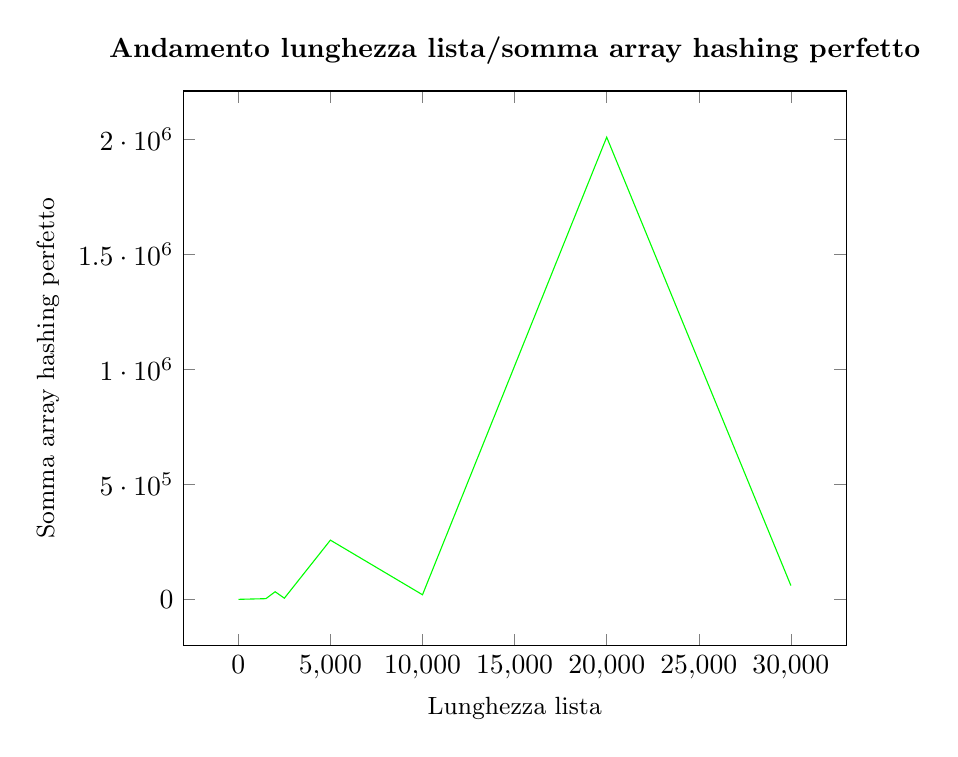
\begin{tikzpicture}
    \begin{axis}[title = {\textbf{Andamento lunghezza lista/somma array hashing perfetto}}, 
        xlabel = \small{Lunghezza lista}, ylabel = \small{Somma array hashing perfetto}, scaled y ticks = false, scaled x ticks = false]
        \addplot[color = green] coordinates{(10, 24)(20, 154)(30, 62)(40, 88)(50, 102)(100, 202)(500, 1006)(1000, 2004)
            (1500, 3002)(2000, 33040)(2500, 5010)(5000, 257550)(10000, 20002)(20000, 2010100)(30000, 60004)};
    \end{axis}
\end{tikzpicture} }
\makebox[\linewidth]{
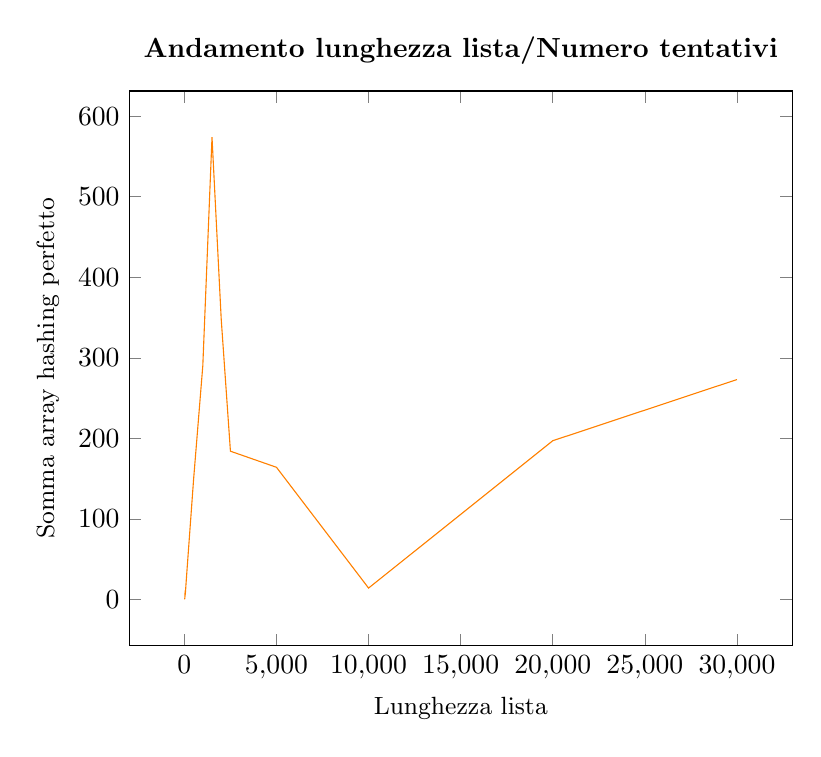
\begin{tikzpicture}
    \begin{axis}[title = {\textbf{Andamento lunghezza lista/Numero tentativi}}, 
        xlabel = \small{Lunghezza lista}, ylabel = \small{Somma array hashing perfetto}, scaled y ticks = false, scaled x ticks = false]
        \addplot[color = orange] coordinates{(10, 0)(20, 1)(30, 3)(40, 11)(50, 6)(100, 23)(500, 149)(1000, 290)(1500, 574)(2000, 348)
            (2500, 184)(5000, 164)(10000, 14)(20000, 197)(30000, 273)};
    \end{axis}
\end{tikzpicture} }    
Come si può notare dai due grafici, non è possibile trarre alcuna correlazione tra il numero di tentativi effettuati e la somma di tutti gli array. 
Però si può notare come, all'aumentare della dimensione della lista, i valori possono essere altalenanti 
(come nel caso della lista di 1500 elementi che ha richiesto 574 tentativi per avere un hash perfetto senza collisioni). 
Da notare anche che è stato imposto il limite della lunghezza della lista a 30000 in quanto è capitato, per quest'ultimo, un tempo di esecuzione superiore ai 5 minuti: 
per questo è stato interrotto forzatamente. Al secondo tentativo di run, infatti, ha elaborato i risultati più velocemente.\\
Riguardo la ricerca, non avendo collisioni, ha complessità $O$(1).

\end{document}